\section{Versuchsaufbau und Messgeräte}

\begin{figure}[htbp]  
     \usetikzlibrary{shapes,arrows}
\tikzstyle{block} = [draw, fill=blue!20, rectangle, 
    minimum height=3em, minimum width=4em]
\tikzstyle{circle} = [draw, fill=blue!20, ellipse, 
    minimum height=2.5em, minimum width=2.5em]
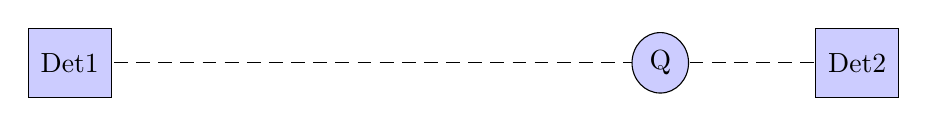
\begin{tikzpicture}
 \coordinate (L) at (-5,0);
 \coordinate (R) at (5,0);
\coordinate (A) at (2.5,4.3);
\coordinate (O) at (2.5,0);

\draw[dash pattern=on5pt off3pt] (L) -- (R);


\node[block, name=det1] at (L) {Det1};
\node[block, name=det2, rotate=0] at (R) {Det2};
\node[circle, name=source] at (O) {Q};

\end{tikzpicture}
  \caption{Schematischer Aufbau zur Energie-Kalibrierung mit der Quelle (Q) $^{22}$Na}
  \label{aufbau1}
\end{figure}

In diesem Versuch werden zwei Detektoren vom Typ NE213 verwendet. Zunächst wird eine Natrium-22-Quelle in der Mitte dieser beiden aufeinander gereichteten Detektoren platziert (siehe Abbildung \ref{aufbau1}). Nach der Kalibrierung wird nun diese Quelle mit einer Americium-241-Berillium-9-Quelle ausgetauscht. Die Absorber, die nun in den Strahlengang zwischen der Quelle und dem Detektor 1 gestellt werden, müssen einen bestimmten Abstand $a$ zu dem Detektor haben (siehe Abbildung \ref{aufbau2}). Die Bedingung dafür ist, dass die Neutronenstrahlen von der Quelle Q (als punktförmig angenommen) die gesamte Länge $l$ des Absorbers durchqueren  müssen, bevor sie den Detektor erreichen. Detektoren und Absorber sind zylinderförmig und die Zylinderachse liegt auf der Strahachse. Aus dem Strahlensatz ergibt sich dann mit dem Abstand Quelle - Detektor $x$, Durchmesser Detektor $D$ und Durchmesser Absorber $d$
\begin{equation}
 \frac{x-a}{d} = \frac{x}{D}
\end{equation}
und dann auch direkt 
\begin{equation}
 a = x\left(1-\frac{d}{D}\right).
\end{equation}

\begin{figure}[htbp]  
     \usetikzlibrary{shapes,arrows}
\tikzstyle{ann} = [fill=white,font=\footnotesize,inner sep=1pt]
\tikzstyle{block} = [draw, fill=blue!20, rectangle, 
    minimum height=2.5em, minimum width=3em]
\tikzstyle{circle} = [draw, fill=blue!20, ellipse, 
    minimum height=0.75em, minimum width=0.75em]
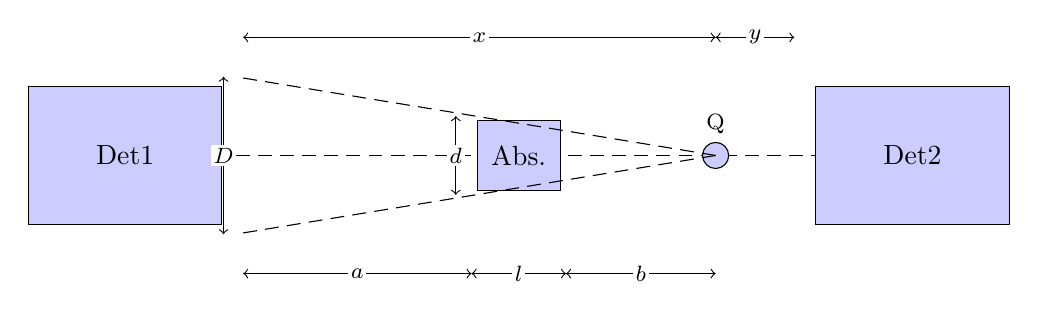
\begin{tikzpicture}
 \coordinate (L) at (-5,0);
 \coordinate (R) at (5,0);
\coordinate (A) at (2.5,4.3);
\coordinate (O) at (2.5,0);

\draw[dash pattern=on5pt off3pt] (L) -- (R);


\node[block, name=det1, minimum height=5em, minimum width=7em] at (L) {Det1};
\node[block, name=det2, minimum height=5em, minimum width=7em, rotate=0] at (R) {Det2};
\node[circle, name=source] at (O) {};
\node[block, name=absorber] at (-0,0){Abs.};

\draw[dash pattern=on5pt off3pt] (O) -- (-3.6,1);
\draw[dash pattern=on5pt off3pt] (O) -- (-3.6,-1);

\draw[arrows=<->](-3.75,1)--(-3.75,-1);
\node[ann] at (-3.75,0) {$D$};

\draw[arrows=<->](-3.5,-1.5)--(-0.6,-1.5);
\node[ann] at (-2.05,-1.5) {$a$};

\draw[arrows=<->](0.6,-1.5)--(-0.6,-1.5);
\node[ann] at (0,-1.5) {$l$};

\draw[arrows=<->](0.6,-1.5)--(2.5,-1.5);
\node[ann] at (1.55,-1.5) {$b$};

\draw[arrows=<->](-0.8,-0.5)--(-0.8,0.5);
\node[ann] at (-0.8,0) {$d$};

\draw[arrows=<->](-3.5,1.5)--(2.5,1.5);
\node[ann] at (-0.5,1.5) {$x$};

\draw[arrows=<->](3.5,1.5)--(2.5,1.5);
\node[ann] at (3,1.5) {$y$};

\node[ann] at (2.5,0.4) {Q};




\end{tikzpicture}
  \caption{Schematischer Aufbau zur Kernradienbestimmung des Absorbers (Abs.) mit der Quelle (Q) $^{241}$Am-$^9$Be}
  \label{aufbau2}
\end{figure}

Mit den Werten $D=11,43 cm$, $d= 4cm$ und $x=50cm$ erhält man $a=32,5 cm$. Da die Länge dea Absorbers $l=5cm$ ist, erhält man für $b=12,5cm$. Für die Time-of-Flight-Messung ist es noch wichtig $y=3,15cm$ zu wissen.

Die Signale aus den Detektoren werden über eine Verstärkerelektronik und einen Analag-Digital-Wandler zum Computer geführt, auf dem die Signale dargestellt werden. Außerdem gibt es einen Zeit-Analysator der Koinzidenzen zwischen den beiden Detektoren erkennt und Zeitdifferenz auf dem Computer darstellt. Als letztes ist das PSD-Signal zu nennen, was in der Elektronik generiert wird und auf dem Computer als 2D-Histogramm dargestellt werden kann.
